\documentclass[11pt,letterpaper]{article}
\usepackage{graphicx}
\usepackage[left=3cm,top=2cm,bottom=2cm,right=3cm]{geometry}
\usepackage[title,titletoc]{appendix}
\usepackage[noblocks]{authblk}
%\usepackage{multirow}
\usepackage{url}
\usepackage{subfigure}
\usepackage{draftwatermark}

% The default is to indent the start of each paragraph.  This is
% annoying and we can disable it with this:
% \setlength\parindent{0pt}

\title{\bf Data Formatter Firmware Design Note}
\author{Yasuyuki Okumura}
\affil{University of Chicago, Chicago, Illinois 60637, USA}
\author{Zihao Jiang}
\affil{Stanford University, Stanford, California, 94305, USA}
\date{\today}

% watermark DRAFT on each page
\SetWatermarkLightness{ 0.95 }
\SetWatermarkScale{ 5 }

\begin{document}
\maketitle

\begin{abstract}
\end{abstract}

\section{Introduction}

This documentation describes the design of the Data Formatter Firmware. 
The development log of DF FW is stored in: \url{https://its.cern.ch/jira/browse/FTKHWD-119}. This version of documentation also summarizes the change of DF FW version change from 18000 to 18022. 

\section{Changes included in this version of note}
\begin{enumerate}

 \item Re-assignment of tower to DF boards to satisfy the requirement from SSB-FLIC so that each DF board outputs two adjacent $\eta$ towers. 
 \item Increase of FW speed from 150 MHz to 200 MHz
 \item Implementation of automatic FMC delay value setting
 \item Automatic retrieval of IP and MAC address using EFUSE USR register
 \item Addition of SLINK output for SSB and implementation of QSFP link for inter-crate DF communication and DF-SSB communication
 \item Dual SLINK output packer structure to improve data formatter speed
 \item SLINK module completion time-out in case of packets loss/corruption in incoming module data or inter-board communication without affecting dataflow
 \item FMC input b0f time-out in case the ID goes busy for a short period of time to disable certain IM input channels without affecting dataflow
 \item Majority L1ID out-of-sync monitoring 
 \item FMC input re-sync functionality (to be validated in data) designed to re-enable input channels b0f timed-out 

\end{enumerate}


\section{32 board allocation and numbering}

Table \ref{tab:shelf1}, \ref{tab:shelf2}, \ref{tab:shelf3} and \ref{tab:shelf4} show DF boards allocation and numbering in USA 15. 


\begin{table}[h]
\centering
\tiny
\begin{tabular}{|c|c|c|c|c|c|c|c|c|}
\hline
Board ID               & bit mask              & \multicolumn{2}{c|}{location}                          & \multicolumn{2}{c|}{destination 1}                            & \multicolumn{2}{c|}{destination 2}                            & \multicolumn{1}{c|}{inter-crate link destination} \\ \hline
\multicolumn{1}{|l|}{} & \multicolumn{1}{l|}{} & \multicolumn{1}{l|}{Shelf} & \multicolumn{1}{l|}{Slot} & \multicolumn{1}{l|}{Tower ID} & \multicolumn{1}{l|}{Position} & \multicolumn{1}{l|}{Tower ID} & \multicolumn{1}{l|}{Position} &                                                   \\ \hline
0                      & 0x00000001            & 1                          & 3                         & 2                             & C E phi1                      & 18                            & C B phi1                      & Shelf 3 - Slot 6                                  \\ \hline
4                      & 0x00000010            & 1                          & 4                         & 3                             & C E phi2                      & 19                            & C B phi2                      & Shelf 4 - Slot 8                                  \\ \hline
8                      & 0x00000100            & 1                          & 5                         & 34                            & A B phi1                      & 50                            & A E phi1                      & Shelf 4 - Slot 9                                  \\ \hline
12                     & 0x00001000            & 1                          & 6                         & 35                            & A B phi2                      & 51                            & A E phi2                      & Shelf 4 - Slot 10                                 \\ \hline
16                     & 0x00010000            & 1                          & 7                         & 4                             & C E phi3                      & 20                            & C B phi3                      & Shelf 2 - Slot 3                                  \\ \hline
20                     & 0x00100000            & 1                          & 8                         & 5                             & C E phi4                      & 21                            & C B phi4                      & Shelf 2 - Slot 4                                  \\ \hline
24                     & 0x01000000            & 1                          & 9                         & 36                            & A B phi3                      & 52                            & A E phi3                      & Shelf 2 - Slot 5                                  \\ \hline
28                     & 0x10000000            & 1                          & 10                        & 37                            & A B phi4                      & 53                            & A E phi4                      & Shelf 2 - Slot 6                                  \\ \hline
\end{tabular}
\caption{Shelf 1.}
\label{tab:shelf1}
\end{table}


\begin{table}[h]
\centering
\tiny
\begin{tabular}{|c|c|c|c|c|c|c|c|c|}
\hline
Board ID               & bit mask              & \multicolumn{2}{c|}{location}                          & \multicolumn{2}{c|}{destination 1}                            & \multicolumn{2}{c|}{destination 2}                            & inter-crate link destination \\ \hline
\multicolumn{1}{|l|}{} & \multicolumn{1}{l|}{} & \multicolumn{1}{l|}{Shelf} & \multicolumn{1}{l|}{Slot} & \multicolumn{1}{l|}{Tower ID} & \multicolumn{1}{l|}{Position} & \multicolumn{1}{l|}{Tower ID} & \multicolumn{1}{l|}{Position} &                              \\ \hline
1                      & 0x00000002            & 2                          & 3                         & 6                             & C E phi5                      & 22                            & C B phi5                      & Shelf 1 - Slot 7             \\ \hline
5                      & 0x00000020            & 2                          & 4                         & 7                             & C B phi5                      & 23                            & C B phi6                      & Shelf 1 - Slot 8             \\ \hline
9                      & 0x00000200            & 2                          & 5                         & 38                            & A B phi5                      & 54                            & A E phi5                      & Shelf 1 - Slot 9             \\ \hline
13                     & 0x00002000            & 2                          & 6                         & 39                            & A B phi6                      & 55                            & A E phi6                      & Shelf 1 - Slot 10            \\ \hline
17                     & 0x00020000            & 2                          & 7                         & 8                             & C E phi7                      & 24                            & C B phi7                      & Shelf 3 - Slot 3             \\ \hline
21                     & 0x00200000            & 2                          & 8                         & 9                             & C B phi7                      & 25                            & C B phi8                      & Shelf 3 - Slot 4             \\ \hline
25                     & 0x02000000            & 2                          & 9                         & 40                            & A B phi7                      & 56                            & A E phi7                      & Shelf 3 - Slot 5             \\ \hline
29                     & 0x20000000            & 2                          & 10                        & 41                            & A B phi8                      & 57                            & A E phi8                      & Shelf 4 - Slot 7             \\ \hline
\end{tabular}
\caption{Shelf 2.}
\label{tab:shelf2}
\end{table}


\begin{table}[h]
\centering
\tiny
\begin{tabular}{|c|c|c|c|c|c|c|c|c|}
\hline
Board ID               & bit mask              & \multicolumn{2}{c|}{location}                          & \multicolumn{2}{c|}{destination 1}                            & \multicolumn{2}{c|}{destination 2}                            & inter-crate link destination \\ \hline
\multicolumn{1}{|l|}{} & \multicolumn{1}{l|}{} & \multicolumn{1}{l|}{Shelf} & \multicolumn{1}{l|}{Slot} & \multicolumn{1}{l|}{Tower ID} & \multicolumn{1}{l|}{Position} & \multicolumn{1}{l|}{Tower ID} & \multicolumn{1}{l|}{Position} & Link 1                       \\ \hline
2                      & 0x00000004            & 3                          & 3                         & 10                            & C E phi9                      & 26                            & C B phi9                      & Shelf 2 - Slot 7             \\ \hline
6                      & 0x00000040            & 3                          & 4                         & 11                            & C E phi10                     & 27                            & C B phi10                     & Shelf 2 - Slot 8             \\ \hline
10                     & 0x00000400            & 3                          & 5                         & 42                            & A B phi9                      & 58                            & A E phi9                      & Shelf 2 - Slot 9             \\ \hline
14                     & 0x00004000            & 3                          & 6                         & 43                            & A B phi10                     & 59                            & A E phi10                     & Shelf 1 - Slot 6             \\ \hline
18                     & 0x00040000            & 3                          & 7                         & 12                            & C E phi11                     & 28                            & C B phi11                     & Shelf 4 - Slot 3             \\ \hline
22                     & 0x00400000            & 3                          & 8                         & 13                            & C E phi12                     & 29                            & C B phi12                     & Shelf 4 - Slot 4             \\ \hline
26                     & 0x04000000            & 3                          & 9                         & 44                            & A B phi11                     & 60                            & A E phi11                     & Shelf 4 - Slot 5             \\ \hline
30                     & 0x40000000            & 3                          & 10                        & 45                            & A B phi12                     & 61                            & A E phi12                     & Shelf 4 - Slot 6             \\ \hline
\end{tabular}
\caption{Shelf 3.}
\label{tab:shelf3}
\end{table}


\begin{table}[]
\centering
\tiny
\caption{Shelf 4.}
\label{tab:shelf4}
\begin{tabular}{|c|c|c|c|c|c|c|c|c|}
\hline
Board ID               & bit mask              & \multicolumn{2}{c|}{location}                          & \multicolumn{2}{c|}{destination 1}                            & \multicolumn{2}{c|}{destination 2}                            & inter-crate link destination \\ \hline
\multicolumn{1}{|l|}{} & \multicolumn{1}{l|}{} & \multicolumn{1}{l|}{Shelf} & \multicolumn{1}{l|}{Slot} & \multicolumn{1}{l|}{Tower ID} & \multicolumn{1}{l|}{Position} & \multicolumn{1}{l|}{Tower ID} & \multicolumn{1}{l|}{Position} & Link 1                       \\ \hline
3                      & 0x00000008            & 4                          & 3                         & 14                            & C E phi13                     & 30                            & C E phi14                     & Shelf 3 - Slot 7             \\ \hline
7                      & 0x00000080            & 4                          & 4                         & 15                            & C E phi14                     & 31                            & C B phi14                     & Shelf 3 - Slot 8             \\ \hline
11                     & 0x00000800            & 4                          & 5                         & 46                            & A B phi13                     & 62                            & A B phi14                     & Shelf 3 - Slot 9             \\ \hline
15                     & 0x00008000            & 4                          & 6                         & 47                            & A B phi14                     & 63                            & A E phi14                     & Shelf 3 - Slot 10            \\ \hline
20                     & 0x00080000            & 4                          & 7                         & 0                             & C E phi15                     & 16                            & C B phi15                     & Shelf 2 - Slot 10            \\ \hline
24                     & 0x00800000            & 4                          & 8                         & 1                             & C E phi0                      & 17                            & C B phi0                      & Shelf 1 - Slot 4             \\ \hline
27                     & 0x08000000            & 4                          & 9                         & 32                            & A B phi15                     & 48                            & A E phi15                     & Shelf 1 - Slot 5             \\ \hline
31                     & 0x80000000            & 4                          & 10                        & 33                            & A B phi0                      & 49                            & A E phi0                      & Shelf 3 - Slot 6             \\ \hline
\end{tabular}
\end{table}

\clearpage


%%%%% FW Overview

\section{Overview of the firmware}

    The DF FW has three main blocks: the main logic, the transceiver and the user interface. The main logic is where the input packets get their destination defined and routed properly. The transceiver is the block that handels the SLINK connections to downstream boards as well as the internal link connections among DFs. The user interfaces defines the logic DF communicating to PC through IPBus and includes the monitoring/config registers. The FW diagram is shown in Fig. \ref{fig:OVERVIEW}


\begin{figure}[h!]
  \centering
  \includegraphics[width=0.80\textwidth,clip,page=3]{figures.pdf}
  \caption{Firmware overview.}
  \label{fig:OVERVIEW}
\end{figure}

%%%%% FW Main logic

\section{Main logic}

The main logic reads the input data from IM boards through FMC interface and stripps of the event headers and trailers and determines the module destination through Input Data Operater (IDO). The headers and trailers are then sent directly to Output Data Operator (ODO), while the modules depending on their destination goes directly to ODO or through Internal Link Input (ILI) and Internal Link Output (ILO) to another DF board. The FW diagram is shown in Fig. \ref{fig:MAIN_LOGIC_OVERVIEW}. Detailed description of each module is presented in the subsections of this section. 

\begin{itemize}
\item FMC interface : \url{data_formatter_top/df_fmc_interface.vhd}
\item Input Data Operator : \url{data_formatter_top/df_input_data_operator.vhd}
\item Output Data Operator : \url{data_formatter_top/df_output_data_operator_v2.vhd}
\item Internal Link Input : \url{data_formatter_top/df_internallink_input.vhd}
\item Internal Link Output : \url{data_formatter_top/df_internallink_output.vhd}
\end{itemize}

\begin{figure}[h!]
  \centering
  \includegraphics[width=0.95\textwidth,clip,page=4]{figures.pdf}
  \caption{Main logic overview.}
  \label{fig:MAIN_LOGIC_OVERVIEW}
\end{figure}

\subsection{FMC interface}

The FMC interface has two maps Input Mapper and Mapper which map the data from FMC links to pre-defined DF input channels splitted into IBL/PIX/SCT lanes. The Front logic then decodes the serial data to form 32 bits data words. FMC TX Interface sends back ``HOLD'', ``RESET'' and ``FREEZE'' signal to IM. 

To establish good phase value for FMC connecter, the Pattern Checker checks on incoming idle words in DF config stage to make sure on the correct idle words (4 different kinds) are reconstructed correctly over a period of 0.1s per channel corresponding to BER=$10e-8$. 

The FMC interface diagram is shown in Fig. \ref{fig:FMC_INTERFACE_OVERVIEW}

\begin{itemize}
\item Input mapper : \url{pulsar2_fmc_interface/fmc_rx_mapper_fmc_to_fpga.vhd}
\item Front : \url{pulsar2_fmc_interface/fmc_rx_front.vhd}
\item Mapper : \url{pulsar2_fmc_interface/fmc_rx_mapper_fpga_to_detword.vhd}
\item Frame : \url{pulsar2_fmc_interface/fmc_rx_frame.vhd}
\item Pattern Checker : \url{pulsar2_fmc_interface/fmc_rx_data_checker_v3.vhd}
\item Elasitc Buffer : \url{fmc_input_buffer/fmc_input_buffer.vhd}
\item FMC TX Interface : \url{pulsar2_fmc_interface/fmc_tx_interface.vhd}
\end{itemize}

\begin{figure}[h!]
  \centering
  \includegraphics[width=0.95\textwidth,clip,page=5]{figures.pdf}
  \caption{FMC interface firmware overview.}
  \label{fig:FMC_INTERFACE_OVERVIEW}
\end{figure}

\subsection{Input data operator}

The IDO (logic shown in Fig. \ref{fig:INPUT_DATA_OPERATOR_OVERVIEW}) connects to ODO and ILO. This FW block strips off the headers and trailers of incoming data (of the first enabled IM channel) sending them through express lane to ODO. The module data goes through a state machine diagrammed in Fig. \ref{fig:STATE_MACHINE_FRAME_ADDER_NORMAL_MODES} for the FW to add on DF internal processing data words (Fig. \ref{fig:INTERNAL_DATA_FORMAT}) and to determine its proper destination. Depending on the destination board of the module would either go directly to the ODO of the current DF board, or will be sent through ILO to another DF. 

A number of special functionalities are implemented to stablize the dataflow in extreme conditions of ID. 
\begin{itemize}
\item \textbf{L1ID out of sync monitoring:} DF implements a seeded majority check of L1ID across all input channels. The seed L1ID is initialized as the first L1ID we receive from the first enabled channel. Then for the subsequent events, we first compare L1ID from all channels to the seed. If we see at least one channel has L1ID that is +1 of the seed, then the seed is incremented. Else if we see at least one channel that sees an ECR then the seed would be set to the ECR. After the seed is determined by all channels, we compare the seed against all L1IDs received and determine which lanes are out of sync. Note the L1ID out of sync monitoring is only for monitoring purpose. We do not disable input channels because of L1ID out of sync.  The code is implemented in \url{pulsar2_df_internal_decoder/df_input_handler.vhd}

\item \textbf{b0f time-out:} As shown in Fig. \ref{fig:STATE_MACHINE_FRAME_ADDER_NORMAL_MODES}, all input channels are required to be synced at the state ``WAIT CHECK HEADER 0 AND SEND DF HEADER''. If one of the enabled channels do not finish the previous event, the signal ``ready\_to\_see\_next\_event'' stays at 0 and hecne all channels are stalled. This design ensures the DF is synced at the input level, while it is not robust against the scenario that a few ID channels going busy and not sending FTK data. Therefore, we inplement a b0f time-out scheme such that we maintain a counter that counts the number of clock cycles since the first channel receivng the ``b0f''. If the counter surpasses a threshold, the channels which have not yet received the ``b0f'' word would be disabled and the ones do will proceed on with the next event. The code is implemented in \url{pulsar2_df_internal_decoder/add_df_internalframe.vhd}

\item \textbf{b0f resync:} If a particular input channel is timed-out, we make an attempt to resync it. Once we see a ``b0f'' word again from the disabled channel, we enter a ``loop'' mode re-enabling and spying on the channel without sending the input data downstream. We start re-processing the channel once we see an ECR that is synchronized with other input channels. The code is implemented in \url{pulsar2_df_internal_decoder/add_df_internalframe.vhd}. NOTE: THIS FUNCTIONALITY HASN'T BEEN FULLY TESTED YET.
\end{itemize}

\begin{itemize}
\item Input lane handler : \url{pulsar2_df_internal_decoder/df_input_handler.vhd}
\item Internal frame adder : \url{pulsar2_df_internal_decoder/add_df_internalframe.vhd}
\item SWITCH : \url{pulsar2_df_switch/df_switch_element_v3.vhd}
\end{itemize}


\begin{figure}[h!]
  \centering
  \includegraphics[width=0.95\textwidth,clip,page=6]{figures.pdf}
  \caption{Internal data operator. One modules have three additional words, header, destination words and trailer.}
  \label{fig:INTERNAL_DATA_FORMAT}
\end{figure}

\begin{figure}[h!]
  \centering
  \includegraphics[width=0.95\textwidth,clip,page=7]{figures.pdf}
  \caption{Input data operator firmware overview.}
  \label{fig:INPUT_DATA_OPERATOR_OVERVIEW}
\end{figure}

\begin{figure}[h!]
  \centering
  \includegraphics[width=0.95\textwidth,clip,page=9]{figures.pdf}
  \caption{State machine in Internal frame adder for normal processing modes.}
  \label{fig:STATE_MACHINE_FRAME_ADDER_NORMAL_MODES}
\end{figure}

\begin{figure}[h!]
  \centering
  \includegraphics[width=0.95\textwidth,clip,page=8]{figures.pdf}
  \caption{State machine in Internal frame adder for different processing modes.}
  \label{fig:STATE_MACHINE_FRAME_ADDER_ALL_MODES}
\end{figure}

\clearpage

\subsection{Output data operator}

The ODO (logic shown in Fig. \ref{fig:OUTPUT_DATA_OPERATOR_OVERVIEW}) connects to ILI and IDO. This FW block gathers module data from all DFs should be routed to one of the destination towers the board is associated with. The DF Output Preparation (has switch in it) block will route the module based on the layer number to the proper SLINK channel. SLINK Packer shown in Fig. \ref{fig:EVENT_SORTING_BUFFER_OLD} and \ref{fig:EVENT_SORTING_BUFFER_NEW} holds the module data in circular buffers. If the module is too early for the current event, it is looped in the circular buffer. 

\begin{itemize}
\item DF Output Preparation : \url{pulsar2_df_internal_decoder/df_output_preparation_v2.vhd}
\item Switch 32 x 32 : \url{pulsar2_df_switch/df_switch_matrix_32x32.vhd}
\item SLINK Packer : \url{pulsar2_df_internal_decoder/df_output_slink_packer_v2.vhd}
\end{itemize}


\begin{table}[h]
\centering
\begin{tabular}{|c|c|c|c|c|c|c|}
\cline{1-3} \cline{5-7}
lane & \multicolumn{2}{c|}{description} &  & lane & \multicolumn{2}{c|}{description} \\ \cline{1-3} \cline{5-7} 
     & type            & channel        &  &      & type           & channel         \\ \cline{1-3} \cline{5-7} 
0    & IM              & ch0 and ch1    &  & 16   & IM             & ch8 and ch9     \\ \cline{1-3} \cline{5-7} 
1    & Fabric          & ch3 p0         &  & 17   & Fabric         & ch3 p1          \\ \cline{1-3} \cline{5-7} 
2    & Fabric          & ch4 p0         &  & 18   & Fabric         & ch4 p1          \\ \cline{1-3} \cline{5-7} 
3    & Fabric          & ch5 p0         &  & 19   & Fabric         & ch5 p1          \\ \cline{1-3} \cline{5-7} 
4    & IM              & ch2 and ch3    &  & 20   & IM             & ch10 and ch11   \\ \cline{1-3} \cline{5-7} 
5    & Fabric          & ch6 p0         &  & 21   & Fabric         & ch6 p1          \\ \cline{1-3} \cline{5-7} 
6    & Fabric          & ch7 p0         &  & 22   & Fabric         & ch7 p1          \\ \cline{1-3} \cline{5-7} 
7    & Fabric          & ch8 p0         &  & 23   & Fabric         & ch8 p1          \\ \cline{1-3} \cline{5-7} 
8    & IM              & ch4 and ch5    &  & 24   & IM             & ch12 and ch13   \\ \cline{1-3} \cline{5-7} 
9    & Fabric          & ch9 po0        &  & 25   & Fabric         & ch9 p1          \\ \cline{1-3} \cline{5-7} 
10   & Fabric          & ch10 p0        &  & 26   & Fabric         & ch10 p1         \\ \cline{1-3} \cline{5-7} 
11   & Fabric          & ch11 p0        &  & 27   & Fabric         & ch11 p1         \\ \cline{1-3} \cline{5-7} 
12   & IM              & ch6 and ch7    &  & 28   & IM             & ch14 and ch15   \\ \cline{1-3} \cline{5-7} 
13   & Fabric          & ch12 p0        &  & 29   & Fabric         & ch12 p1         \\ \cline{1-3} \cline{5-7} 
14   & Inter-crate     & ch0 p0         &  & 30   & Inter-crate    & ch0 p1          \\ \cline{1-3} \cline{5-7} 
15   & Inter-crate     & ch1 p0         &  & 31   & Inter-crate    & ch1 p1          \\ \cline{1-3} \cline{5-7} 
\end{tabular}
\caption{Input channel assignment for output data operator module. Defined in 
``MAPPING\_CONF\_IDO2ODO'' and ``MAPPING\_CONF\_ILI2ODO'' in data\_formatter\_top/data\_formatter\_constants.vhd.}
\end{table}


\begin{table}[h]
\centering
\begin{tabular}{|c|c|c|c|c|c|c|}
\cline{1-3} \cline{5-7}
lane & \multicolumn{2}{c|}{description} &  & lane & \multicolumn{2}{c|}{description} \\ \cline{1-3} \cline{5-7} 
     & type              & channel      &  &      & type              & channel      \\ \cline{1-3} \cline{5-7} 
0    & AUX0 Tower 0      & ch0          &  & 17   & AUX0 Tower 1      & ch0          \\ \cline{1-3} \cline{5-7} 
1    & AUX0 Tower 0      & ch1          &  & 18   & AUX0 Tower 1      & ch1          \\ \cline{1-3} \cline{5-7} 
2    & AUX0 Tower 0      & ch2          &  & 19   & AUX0 Tower 1      & ch2          \\ \cline{1-3} \cline{5-7} 
3    & AUX0 Tower 0      & ch3          &  & 20   & AUX0 Tower 1      & ch3          \\ \cline{1-3} \cline{5-7} 
4    & AUX1 Tower 0      & ch4          &  & 21   & AUX1 Tower 1      & ch4          \\ \cline{1-3} \cline{5-7} 
5    & AUX1 Tower 0      & ch5          &  & 22   & AUX1 Tower 1      & ch5          \\ \cline{1-3} \cline{5-7} 
6    & AUX1 Tower 0      & ch6          &  & 23   & AUX1 Tower 1      & ch6          \\ \cline{1-3} \cline{5-7} 
7    & AUX1 Tower 0      & ch7          &  & 24   & AUX1 Tower 1      & ch7          \\ \cline{1-3} \cline{5-7} 
8    & AUX2 Tower 0      & ch0          &  & 25   & AUX2 Tower 1      & ch0          \\ \cline{1-3} \cline{5-7} 
9    & AUX2 Tower 0      & ch1          &  & 26   & AUX2 Tower 1      & ch1          \\ \cline{1-3} \cline{5-7} 
10   & AUX2 Tower 0      & ch2          &  & 27   & AUX2 Tower 1      & ch2          \\ \cline{1-3} \cline{5-7} 
11   & AUX2 Tower 0      & ch3          &  & 28   & AUX2 Tower1       & ch3          \\ \cline{1-3} \cline{5-7} 
12   & AUX3 Tower 0      & ch4          &  & 29   & AUX3 Tower1       & ch4          \\ \cline{1-3} \cline{5-7} 
13   & AUX3 Tower 0      & ch5          &  & 30   & AUX3 Tower1       & ch5          \\ \cline{1-3} \cline{5-7} 
14   & AUX3 Tower 0      & ch6          &  & 31   & AUX3 Tower1       & ch6          \\ \cline{1-3} \cline{5-7} 
15   & AUX3 Tower 0      & ch7          &  & 32   & AUX3 Tower 1      & ch7          \\ \cline{1-3} \cline{5-7} 
16   & SSB Tower 0       &              &  & 33   & SSB Tower 1       &              \\ \cline{1-3} \cline{5-7} 
\end{tabular}
\caption{SLINK output channel assignment (34 channel). 
``MAPPING\_CONF\_SLINKOUT2GTLOC'' and ``MAPPING\_CONF\_SLINKOUT2GTLOC'' in data\_formatter\_top/data\_formatter\_constants.vhd.}
\end{table}


\begin{figure}[h!]
  \centering
  \includegraphics[width=0.95\textwidth,clip,page=10]{figures.pdf}
  \caption{Output data operator firmware overview.}
  \label{fig:OUTPUT_DATA_OPERATOR_OVERVIEW}
\end{figure}

\begin{figure}[h!]
  \centering
  \includegraphics[width=0.95\textwidth,clip,page=11]{figures.pdf}
  \caption{Schematics of the early design of individual event sorting buffer in the SLINK packer. In the current design of DF FW, we have two event sorting buffers for each of the output lane for sorting odd and even numbered events separetely to increase the processing speed. Each sorting buffer is of 4K word size.}
  \label{fig:EVENT_SORTING_BUFFER_OLD}
\end{figure}

\begin{figure}[h!]
  \centering
  \includegraphics[width=0.95\textwidth,clip,page=12]{figures.pdf}
  \caption{Schematics of the current design of individual event sorting buffer in the SLINK packer. The current design strips off the express lane for modules of the current to save FW resources.}
  \label{fig:EVENT_SORTING_BUFFER_NEW}
\end{figure}


\clearpage 

\subsection{Internal link input / output}

The ILI and ILO (\ref{fig:EVENT_INTERNALINK_INOUT}) are blocks for DF-DF communication. The ILO has two 32x32 switches. The first one is CW (central switch) which spreads out the traffic by randomly routing the modules based on the random counter they receive in IDO. The second switch then routes the module to the proper trasceiver. ILI connected to another board's ILO will determine if the module goes out from the current board or needs to be routed again. Hence the ILI connects ODO as well as ILO. 

It is a good exercise for the reader given the information of the DF-DF connection in Tab. \ref{tab:shelf1},\ref{tab:shelf2},\ref{tab:shelf3},\ref{tab:shelf4} to reach the same conclusion as the authors that the there are three different data sharing patterns as show in Fig.\ref{fig:DATA_SHARING_PATTERN}. In practice, the bottle-neck of DF processing is coming from the ODO circular buffer, which origninates from the fact that modules from old and new events need to be cycled through the buffer before an event can be completed. To minimize the overlapping of old and new events, we need to minimize amount of module data being shared in between DFs. A good heruistic is to optimizatize the DF cabling reduce the total path cost of all modules being routed in the DF system. As of how this is done in code level is beyond the scope of this note, please contact Zihao directly for more information. 

The internal link interface (Fig. \ref{fig:EVENT_INTERNALINK}) implements a DF-DF sync scheme. By checking the DF internal event numbers of the incoming events, the destination board determines if it is processing ahead more than 2 events the source board does. The scheme is enforced by the idle words which contain the DF internal current event ID counter sent every 128 cycles (Table. \ref{tab:internallinkidle}). 

\begin{itemize}
\item Internal link interface : \url{pulsar2_df_internal_link/ilink_interface_v2.vhd}
\item Bit Error Rate Test (BERT) pattern generator : \url{pulsar2_df_internal_link/pattern_gen.vhd}
\item Bit Error Rate Test (BERT) pattern checker : \url{pulsar2_df_internal_link/pattern_chk.vhd}
\end{itemize}


\begin{table}[h]
\centering
\begin{tabular}{|c|c|c|c|c|c|c|}
\cline{1-3} \cline{5-7}
lane & \multicolumn{2}{c|}{description} &  & lane & \multicolumn{2}{c|}{description} \\ \cline{1-3} \cline{5-7} 
     & type            & channel        &  &      & type           & channel         \\ \cline{1-3} \cline{5-7} 
0    & IM              & ch0 and ch1    &  & 16   & IM             & ch8 and ch9     \\ \cline{1-3} \cline{5-7} 
1    & Fabric          & ch3 p0         &  & 17   & Fabric         & ch3 p1          \\ \cline{1-3} \cline{5-7} 
2    & Fabric          & ch4 p0         &  & 18   & Fabric         & ch4 p1          \\ \cline{1-3} \cline{5-7} 
3    & Fabric          & ch5 p0         &  & 19   & Fabric         & ch5 p1          \\ \cline{1-3} \cline{5-7} 
4    & IM              & ch2 and ch3    &  & 20   & IM             & ch10 and ch11   \\ \cline{1-3} \cline{5-7} 
5    & Fabric          & ch6 p0         &  & 21   & Fabric         & ch6 p1          \\ \cline{1-3} \cline{5-7} 
6    & Fabric          & ch7 p0         &  & 22   & Fabric         & ch7 p1          \\ \cline{1-3} \cline{5-7} 
7    & Fabric          & ch8 p0         &  & 23   & Fabric         & ch8 p1          \\ \cline{1-3} \cline{5-7} 
8    & IM              & ch4 and ch5    &  & 24   & IM             & ch12 and ch13   \\ \cline{1-3} \cline{5-7} 
9    & Fabric          & ch9 po0        &  & 25   & Fabric         & ch9 p1          \\ \cline{1-3} \cline{5-7} 
10   & Fabric          & ch10 p0        &  & 26   & Fabric         & ch10 p1         \\ \cline{1-3} \cline{5-7} 
11   & Fabric          & ch11 p0        &  & 27   & Fabric         & ch11 p1         \\ \cline{1-3} \cline{5-7} 
12   & IM              & ch6 and ch7    &  & 28   & IM             & ch14 and ch15   \\ \cline{1-3} \cline{5-7} 
13   & Fabric          & ch12 p0        &  & 29   & Fabric         & ch12 p1         \\ \cline{1-3} \cline{5-7} 
14   & Inter-crate     & ch0 p0         &  & 30   & Inter-crate    & ch0 p1          \\ \cline{1-3} \cline{5-7} 
15   & Inter-crate     & ch1 p0         &  & 31   & Inter-crate    & ch1 p1          \\ \cline{1-3} \cline{5-7} 
\end{tabular}
\caption{Input channel assignment for internal data output module (i.e. input of Central Switch.). Defined in 
``MAPPING\_CONF\_IDO2ILO'' and ``MAPPING\_CONF\_ILI2ILO'' in data\_formatter\_top/data\_formatter\_constants.vhd.}
\end{table}

\begin{table}[h]
\centering
\begin{tabular}{|c|c|c|c|c|c|c|}
\cline{1-3} \cline{5-7}
lane & \multicolumn{2}{c|}{description} &  & lane & \multicolumn{2}{c|}{description} \\ \cline{1-3} \cline{5-7} 
     & type               & channel     &  &      & type               & channel     \\ \cline{1-3} \cline{5-7} 
0    & Fabric             & ch3 p0      &  & 12   & Fabric             & ch3 p1      \\ \cline{1-3} \cline{5-7} 
1    & Fabric             & ch4 p0      &  & 13   & Fabric             & ch4 p1      \\ \cline{1-3} \cline{5-7} 
2    & Fabric             & ch5 p0      &  & 14   & Fabric             & ch5 p1      \\ \cline{1-3} \cline{5-7} 
3    & Fabric             & ch6 p0      &  & 15   & Fabric             & ch6 p1      \\ \cline{1-3} \cline{5-7} 
4    & Fabric             & ch7 p0      &  & 16   & Fabric             & ch7 p1      \\ \cline{1-3} \cline{5-7} 
5    & Fabric             & ch8 p0      &  & 17   & Fabric             & ch8 p1      \\ \cline{1-3} \cline{5-7} 
6    & Fabric             & ch9 p0      &  & 18   & Fabric             & ch9 p1      \\ \cline{1-3} \cline{5-7} 
7    & Fabric             & ch10 p0     &  & 19   & Fabric             & ch10 p1     \\ \cline{1-3} \cline{5-7} 
8    & Fabric             & ch11 p0     &  & 20   & Fabric             & ch11 p1     \\ \cline{1-3} \cline{5-7} 
9    & Fabric             & ch12 p0     &  & 21   & Fabric             & ch12 p1     \\ \cline{1-3} \cline{5-7} 
10   & Internal link      & ch0 p0      &  & 22   & Internal link      & ch0 p1      \\ \cline{1-3} \cline{5-7} 
11   & Internal link      & ch1 p0      &  & 23   & Internal link      & ch1 p1      \\ \cline{1-3} \cline{5-7} 
\end{tabular}
\caption{Internal link channel assignment. Defined in 
``MAPPING\_CONF\_INTERNALLINK2GTCHANNEL'' and ``MAPPING\_CONF\_INTERNALLINK2GTLOC'' in data\_formatter\_top/data\_formatter\_constants.vhd.}
\end{table}

\begin{table}[h]
\begin{tabular}{|c|}
\hline
31:0   \\ \hline
$K23.7\&K23.7\&K23.7\&K23.7$ \\ \hline
\end{tabular}
\caption{Pad-word definition. It will be inserted in the interface (TX side) every 128-word cycle, and removed in the interface (RX side) in The isKCharctor word is $1111$. This is for RX clock correction functionality.}
\end{table}

\begin{table}[h]
\begin{tabular}{|c|c|c|c|c|c|}
\hline
31:24 &23:16              & 15:13    & 12   & 11:8                 & 7:0   \\ \hline
$D5.6$ & $00$ Current Event ID & Reserved & XOFF & Return Channel 4 bit & $K28.5$ \\ \hline
\end{tabular}
\label{tab:internallinkidle}
\caption{idle word definition. At least it will be inserted in the interface every 128-word cycle. The isKCharctor word is $0001$.}
\end{table}

\begin{figure}[h!]
  \centering
  \includegraphics[width=0.95\textwidth,clip,page=13]{figures.pdf}
  \caption{Internal link interface. This includes clock domain crossing (CDC) buffer between GT user clocks and main logic clock.}
  \label{fig:EVENT_INTERNALINK}
\end{figure}

\begin{figure}[h!]
  \centering
  \includegraphics[width=0.95\textwidth,clip,page=14]{figures.pdf}
  \caption{Schematics of input and output internal link.}
  \label{fig:EVENT_INTERNALINK_INOUT}
\end{figure}


\begin{figure}[h!]
  \centering
  \includegraphics[width=0.95\textwidth,clip,page=15]{figures.pdf}
  \caption{DF sharing pattern.}
  \label{fig:DATA_SHARING_PATTERN}
\end{figure}


\clearpage

\appendix

\section{ATCA fabric interface}
\begin{figure}[h!]
  \centering
  \includegraphics[width=1.0\textwidth,clip,page=16]{figures.pdf}
  \caption{ATCA fabric connection table.}
  \label{fig:ATCAFabricConnectionTable}
\end{figure}

\section{GT channel assignment}
\begin{figure}[h!]
  \centering
  \includegraphics[width=1.0\textwidth,clip,page=17]{figures.pdf}
  \caption{Transceiver channel assignment summary (1). For RTM channels.}
  \label{fig:GTChannel1}
\end{figure}

\begin{figure}[h!]
  \centering
  \includegraphics[width=1.0\textwidth,clip,page=18]{figures.pdf}
  \caption{Transceiver channel assignment summary (2). For Fabric and DF-IM channels.}
  \label{fig:GTChannel2}
\end{figure}

\newpage
\clearpage 

\section {IP Bus registers}

See \url{https://okumura.web.cern.ch/okumura/tmp/address_df.xml}. 
\subsection {IP Address}

\begin{table}[h!]
\centering
\begin{tabular}{|l|l|l|l|l|}
\hline
Address  & Bit Postion & R/W & Name & Description \\ \hline
0X00000000           & 31:0        & R   & ipaddress & IP address (IPv4 32 bit)  \\ \hline
\end{tabular}
\end{table}

\subsection {Reset}

\begin{table}[h!]
\centering
\begin{tabular}{|l|l|l|l|l|}
\hline
Address  & Bit Postion & R/W & Name  & Description \\ \hline
0X00000001           &             &     & reset &   \\ \hline
                     & 0           & R/W & reset\_delay &  \\ \hline
                     & 1           & R/W & disable\_fmc\_input &  \\ \hline
                     & 2           & R/W & reset\_parity\_checker &  \\ \hline
                     & 3           & R/W & fmcin\_logic\_reset &  \\ \hline
                     & 4           & R/W & main\_state\_machine\_reset  &  \\ \hline
                     & 5           & R/W & i2c\_state\_machine\_reset &  \\ \hline
                     & 6           & R/W & configurable\_parameter\_reset &  \\ \hline
                     & 7           & R/W & counter\_parameter\_reset &  \\ \hline
                     & 8           & R/W & counter\_parameter\_reset &  \\ \hline
                     & 31:9        &  -  & & Reserved  \\ \hline
\end{tabular}
\end{table}

\subsection {Front FIFO error}

\begin{table}[h!]
\centering
\begin{tabular}{|l|l|l|l|l|}
\hline
Address  & Bit Postion & R/W & Name  & Description \\ \hline
0X00000002           &             & R    & fmcin\_front\_fifo\_error &   \\ \hline
\end{tabular}
\end{table}


.... to be summarized, including the details of use case for all the parameters.

\end{document}
